\section{TinyML Model Performance}
\label{sec:ch4-tinyml-model-performance}

The TinyML results were interpreted at two levels. First, the embedded
prototype was evaluated by trial-level relay behavior in the laboratory.
Second, the exported Random Forest report was evaluated by held-out
frame-level and event-level metrics. Both views are useful: trial-level
behavior reflects the complete protection sequence, while frame-level metrics
show how the model performed before relay-counter persistence.

Table~\ref{tab:ch4-trial-metrics} gives the trial-level metrics for
recognized loads, unrecognized loads, and all loads combined.
\begin{table}[H]
  \centering
  \caption{Trial-level arc-fault performance metrics}
  \label{tab:ch4-trial-metrics}
  \begin{tabular}{lcccc}
    \toprule
    \textbf{Load group} & \textbf{Accuracy} & \textbf{Precision} & \textbf{Recall} & \textbf{F1-score} \\
    \midrule
    Recognized loads & 99.00\% & 100.00\% & 98.00\% & 98.99\% \\
    Unrecognized loads & 96.00\% & 97.92\% & 94.00\% & 95.92\% \\
    All tested loads & 97.50\% & 98.97\% & 96.00\% & 97.46\% \\
    \bottomrule
  \end{tabular}
\end{table}

Figure~\ref{fig:ch4-group-metrics} graphs the same four metrics by load
setup. This presentation compares like quantities across recognized,
unrecognized, and combined test groups; it does not mix unrelated metrics as
separate one-off bars.
\begin{figure}[H]
  \centering
  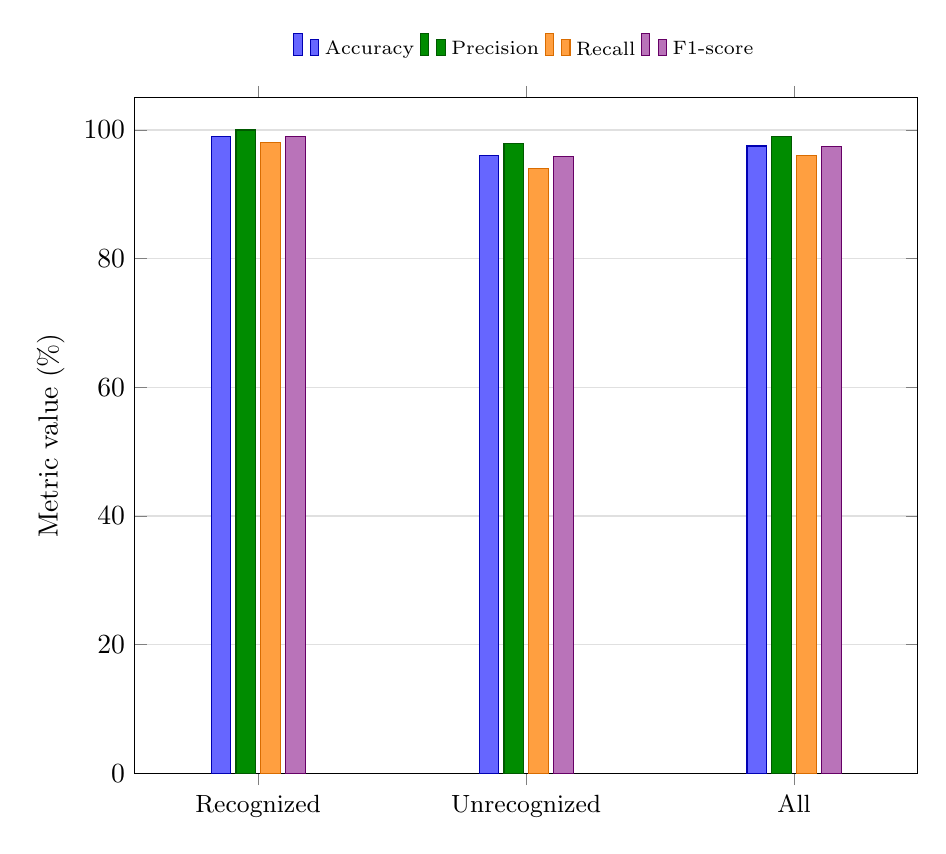
\begin{tikzpicture}
    \begin{axis}[
      ybar,
      width=0.95\textwidth,
      height=4in,
      ymin=0,
      ymax=105,
      ylabel={Metric value (\%)},
      symbolic x coords={Recognized,Unrecognized,All},
      xtick=data,
      x tick label style={font=\small},
      ymajorgrids=true,
      grid style={black!12},
      bar width=7pt,
      enlarge x limits=0.23,
      legend style={font=\scriptsize,at={(0.5,1.04)},anchor=south,legend columns=4,draw=none},
      legend cell align={left}
    ]
      \addplot[fill=blue!60,draw=blue!70!black] coordinates {(Recognized,99.00) (Unrecognized,96.00) (All,97.50)};
      \addplot[fill=green!55!black,draw=green!35!black] coordinates {(Recognized,100.00) (Unrecognized,97.92) (All,98.97)};
      \addplot[fill=orange!75,draw=orange!85!black] coordinates {(Recognized,98.00) (Unrecognized,94.00) (All,96.00)};
      \addplot[fill=violet!55,draw=violet!80!black] coordinates {(Recognized,98.99) (Unrecognized,95.92) (All,97.46)};
      \legend{Accuracy,Precision,Recall,F1-score}
    \end{axis}
  \end{tikzpicture}
  \caption{Trial-level performance metrics by recognized and unrecognized load setup.}
  \label{fig:ch4-group-metrics}
\end{figure}

Table~\ref{tab:ch4-trial-metrics} and Figure~\ref{fig:ch4-group-metrics} show
high overall performance across 200 trial outcomes. Precision is related to
nuisance trips: the 98.97\% overall precision means that only one normal
event was incorrectly tripped in the trial set. Recall is related to safety
sensitivity: the 96.00\% overall recall means that four arc trials were
missed. The recognized-load group had slightly higher recall and no
normal-event false trip, while the unrecognized-load group accounted for
three of the four missed arc trials and the single false trip. This indicates
that the deployed model generalized reasonably, but the unrecognized load
cases remained the more difficult condition.

The trial-level classifier and persistence logic produced balanced
performance: precision remained high for nuisance-trip reduction, while recall
remained high enough to detect most arc trials. These results apply to the
deployed feature contract described in Section~\ref{sec:ch3-feature-contract}:
six selected waveform features were used by the arc model, with context fields
appended to the model vector.

The per-load trial metrics are shown in Table~\ref{tab:ch4-per-load-metrics}.
\begin{table}[H]
  \centering
  \caption{Per-load trial-level performance metrics}
  \label{tab:ch4-per-load-metrics}
  \small
  \setlength{\tabcolsep}{2.5pt}
  \begin{tabular}{p{0.24\textwidth}p{0.15\textwidth}cccc}
    \toprule
    \textbf{Device} & \textbf{Device type} & \textbf{Accuracy} & \textbf{Precision} & \textbf{Recall} & \textbf{F1-score} \\
    \midrule
    Water heater & Resistive & 100\% & 100\% & 100\% & 100\% \\
    Halogen lamp & Resistive & 100\% & 100\% & 100\% & 100\% \\
    Electric kettle & Resistive & 100\% & 100\% & 100\% & 100\% \\
    40W stand fan & Inductive & 100\% & 100\% & 100\% & 100\% \\
    Handheld vacuum & Brushed & 95\% & 100\% & 90\% & 94.74\% \\
    Electrolux vacuum & Brushed & 95\% & 100\% & 90\% & 94.74\% \\
    Angle grinder & Brushed & 95\% & 100\% & 90\% & 94.74\% \\
    Bench cutter & Brushed & 95\% & 100\% & 90\% & 94.74\% \\
    Impact drill & Brushed & 95\% & 90.91\% & 100\% & 95.24\% \\
    Heat gun & Resistive & 100\% & 100\% & 100\% & 100\% \\
    \bottomrule
  \end{tabular}
\end{table}

Table~\ref{tab:ch4-per-load-metrics} shows where the group-level metrics came
from without adding another graph below it. The impact drill is the only load
listed with precision below 100\%, meaning it contributed the normal-event
false trip. The handheld vacuum, vacuum cleaner, angle grinder, and bench
cutter had lower recall, meaning those load cases contributed missed arc
trials.

The same appendix data can also be aggregated by load setup and load family.
For load setup, recognized loads contributed 49 detected arc trials, one
missed arc trial, 50 correct normal trials, and no false trip; unrecognized
loads contributed 47 detected arc trials, three missed arc trials, 49 correct
normal trials, and one false trip. For family grouping, water heater, halogen
lamp, electric kettle, and heat gun were treated as resistive loads; the 40W
stand fan was treated as the inductive load; and the handheld vacuum,
Electrolux vacuum, angle grinder, bench cutter, and impact drill were
treated as brushed or universal-motor loads. These aggregations summarize the
recorded trial tables in Appendix~\ref{app:e}; they are not additional test
conditions.
\begin{figure}[H]
  \centering
  \begin{minipage}{0.47\textwidth}
    \centering
    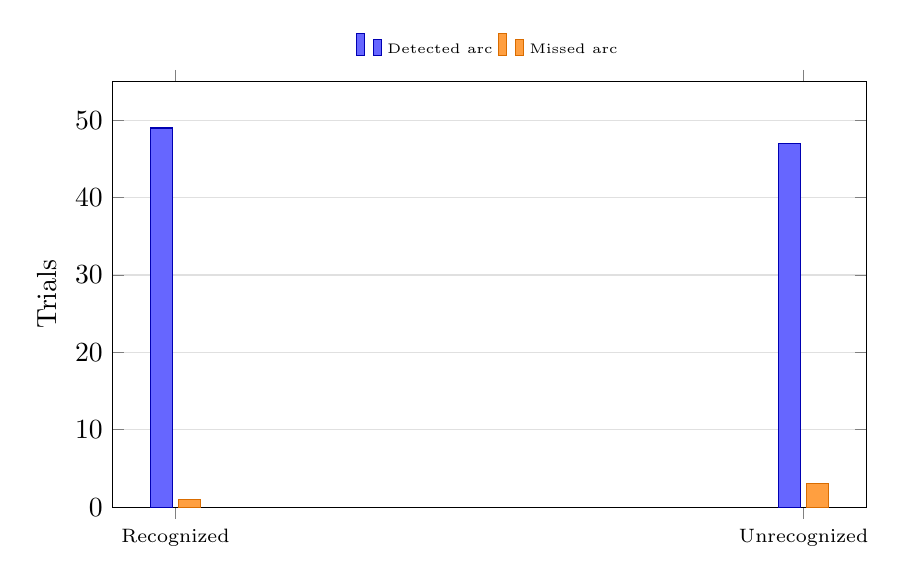
\begin{tikzpicture}
      \begin{axis}[
        ybar,
        width=0.92\linewidth,
        height=2.75in,
        ymin=0,
        ymax=55,
        ylabel={Trials},
        symbolic x coords={Recognized,Unrecognized},
        xtick=data,
        x tick label style={font=\scriptsize},
        ymajorgrids=true,
        grid style={black!12},
        bar width=8pt,
        legend style={font=\tiny,at={(0.5,1.03)},anchor=south,legend columns=2,draw=none},
      ]
        \addplot[fill=blue!60,draw=blue!70!black] coordinates {(Recognized,49) (Unrecognized,47)};
        \addplot[fill=orange!75,draw=orange!85!black] coordinates {(Recognized,1) (Unrecognized,3)};
        \legend{Detected arc,Missed arc}
      \end{axis}
    \end{tikzpicture}
    {\small (a) Arc Trials}
  \end{minipage}\hfill
  \begin{minipage}{0.47\textwidth}
    \centering
    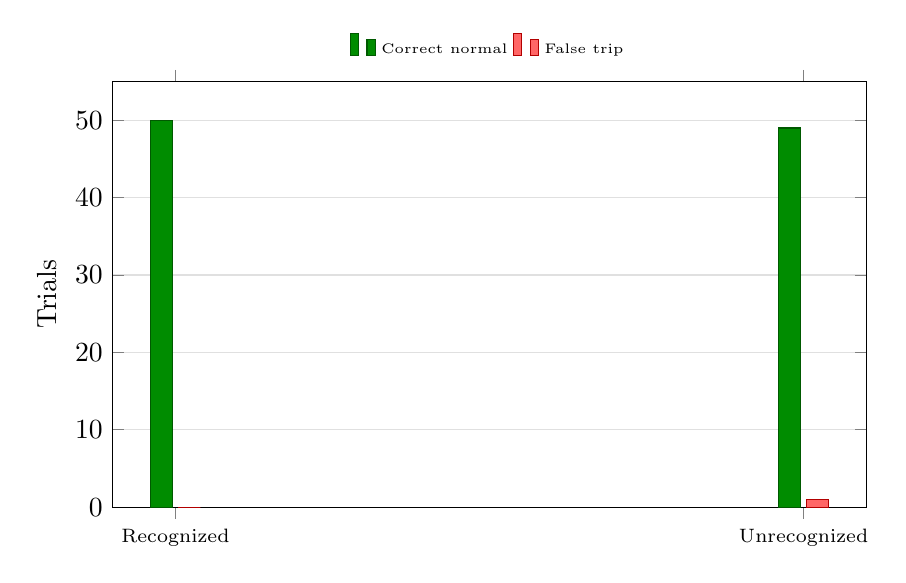
\begin{tikzpicture}
      \begin{axis}[
        ybar,
        width=0.92\linewidth,
        height=2.75in,
        ymin=0,
        ymax=55,
        ylabel={Trials},
        symbolic x coords={Recognized,Unrecognized},
        xtick=data,
        x tick label style={font=\scriptsize},
        ymajorgrids=true,
        grid style={black!12},
        bar width=8pt,
        legend style={font=\tiny,at={(0.5,1.03)},anchor=south,legend columns=2,draw=none},
      ]
        \addplot[fill=green!55!black,draw=green!35!black] coordinates {(Recognized,50) (Unrecognized,49)};
        \addplot[fill=red!60,draw=red!70!black] coordinates {(Recognized,0) (Unrecognized,1)};
        \legend{Correct normal,False trip}
      \end{axis}
    \end{tikzpicture}
    {\small (b) Normal Trials}
  \end{minipage}
  \caption{Grouped trial outcomes for recognized and unrecognized load setups.}
  \label{fig:ch4-setup-outcomes}
\end{figure}

Figure~\ref{fig:ch4-setup-outcomes}(a) shows that the unrecognized group had
more missed arc trials than the recognized group. Figure~\ref{fig:ch4-setup-outcomes}(b)
shows that the only normal-event false trip also came from the unrecognized
group. These results are consistent with the per-load results in
Table~\ref{tab:ch4-per-load-metrics}: generalization loads were still handled
by the protection sequence, but they produced the remaining errors.

\begin{figure}[H]
  \centering
  \begin{minipage}{0.47\textwidth}
    \centering
    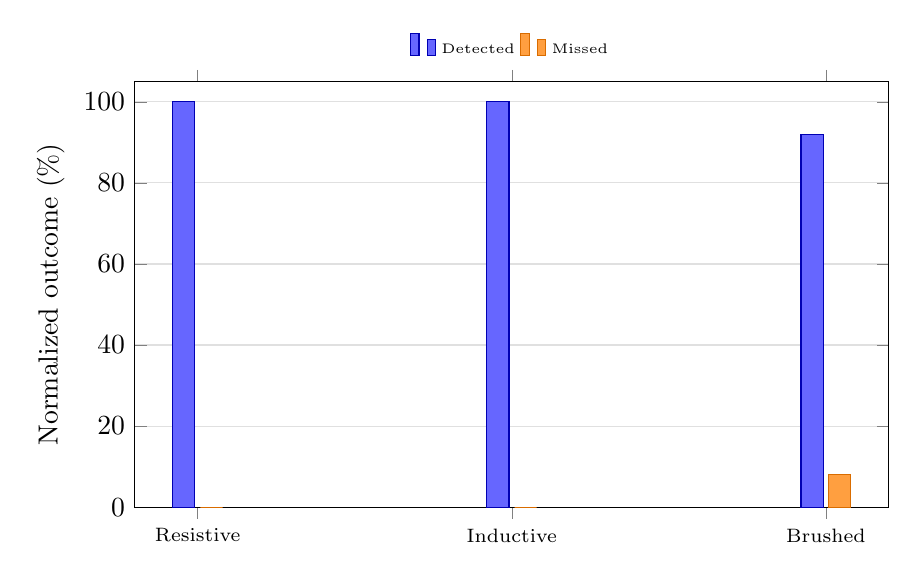
\begin{tikzpicture}
      \begin{axis}[
        ybar,
        width=0.92\linewidth,
        height=2.75in,
        ymin=0,
        ymax=105,
        ylabel={Normalized outcome (\%)},
        symbolic x coords={Resistive,Inductive,Brushed},
        xtick=data,
        x tick label style={font=\scriptsize},
        ymajorgrids=true,
        grid style={black!12},
        bar width=8pt,
        legend style={font=\tiny,at={(0.5,1.03)},anchor=south,legend columns=2,draw=none},
      ]
        \addplot[fill=blue!60,draw=blue!70!black] coordinates {(Resistive,100) (Inductive,100) (Brushed,92)};
        \addplot[fill=orange!75,draw=orange!85!black] coordinates {(Resistive,0) (Inductive,0) (Brushed,8)};
        \legend{Detected,Missed}
      \end{axis}
    \end{tikzpicture}
    {\small (a) Arc Trials}
  \end{minipage}\hfill
  \begin{minipage}{0.47\textwidth}
    \centering
    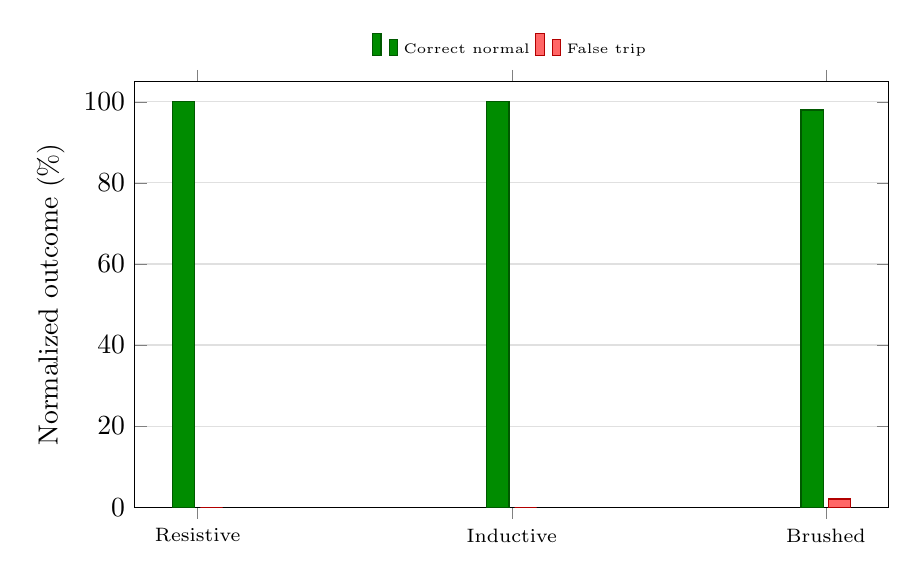
\begin{tikzpicture}
      \begin{axis}[
        ybar,
        width=0.92\linewidth,
        height=2.75in,
        ymin=0,
        ymax=105,
        ylabel={Normalized outcome (\%)},
        symbolic x coords={Resistive,Inductive,Brushed},
        xtick=data,
        x tick label style={font=\scriptsize},
        ymajorgrids=true,
        grid style={black!12},
        bar width=8pt,
        legend style={font=\tiny,at={(0.5,1.03)},anchor=south,legend columns=2,draw=none},
      ]
        \addplot[fill=green!55!black,draw=green!35!black] coordinates {(Resistive,100) (Inductive,100) (Brushed,98)};
        \addplot[fill=red!60,draw=red!70!black] coordinates {(Resistive,0) (Inductive,0) (Brushed,2)};
        \legend{Correct normal,False trip}
      \end{axis}
    \end{tikzpicture}
    {\small (b) Normal Trials}
  \end{minipage}
  \caption{Normalized grouped trial outcomes by load family.}
  \label{fig:ch4-family-outcomes}
\end{figure}

Figure~\ref{fig:ch4-family-outcomes} is normalized because the family groups
did not contain the same number of devices or trials. In
Figure~\ref{fig:ch4-family-outcomes}(a), resistive and inductive load-family
trials had 100\% arc detection, while the brushed-load family had 92\%
arc detection and 8\% missed arc trials. In
Figure~\ref{fig:ch4-family-outcomes}(b), the brushed-load family also
contained the only false trip, giving 98\% correct normal classification and
2\% false-trip outcome for that family. The normalized view therefore shows
that the brushed or universal-motor group was the main source of residual
model error rather than simply the largest group in raw counts.

The exported Random Forest report provides a second view of performance.
The held-out test split contained 10,268 feature rows, including 90 positive
rows. The frame-level confusion matrix contained 10,173 true negatives, 5
false positives, 25 false negatives, and 65 true positives. The corresponding
frame-level accuracy was 99.7078\%, precision was 92.8571\%, recall was
72.2222\%, and F1-score was 81.25\%. At event level, the same report showed
25 true arc events, 21 detected events, 4 missed events, 31 predicted events,
1 false-alarm event, 84.0\% event recall, 96.7742\% event precision, and
89.9358\% event F1-score. The data-preparation, training-report, and
exported-model details supporting these metrics are summarized in
Appendix~\ref{app:f-tinyml-training-summary}.

These model-report values are lower than the final trial-level relay metrics
because they evaluate individual frames and event groupings before the full
trial-level interpretation. This does not invalidate the trial results; it
shows that the firmware's persistence logic is part of the protection
behavior. The deployed model should therefore be judged as a
model-plus-firmware system, not as a standalone frame classifier.

\section{Model Limitations}
\label{sec:ch4-model-limitations}

The main limitation is dataset coverage. The tests included recognized and
unrecognized loads, but they did not cover all appliance families, wiring
conditions, electrode materials, contact gaps, ambient conditions, or utility
waveform variations. The results therefore support prototype feasibility and
future development, but they do not establish compliance with AFCI standards
or replacement equivalence with certified protective devices.
